\documentclass[12pt, letterpaper]{article}
\usepackage{fullpage}
\usepackage[top=1cm, bottom=4cm, left=2cm, right=2cm]{geometry}
\usepackage{amsmath,amsthm,amsfonts,amssymb,amscd}
\usepackage{lastpage}
\usepackage{enumerate}
\usepackage{fancyhdr}
\usepackage{mathrsfs}
\usepackage{graphicx}
%% download this package and put it in the same directory as this file
\setlength{\parindent}{0.0in}
\setlength{\parskip}{0.2cm}
\graphicspath{ {../figures/} }
\usepackage{subfigure}
\usepackage{float}
\usepackage{multicol}
\usepackage{multirow}
\usepackage{enumitem}
% Edit these as appropriate
\newcommand\course{DATA1030}
\newcommand\semester{Fall 2020}
\newcommand\Name{Ben Xiong}           % <-- Fill in your name here
\usepackage{lettrine}
\pagestyle{fancyplain}
\headheight 35pt
\fancyfoot{}
\lhead{\Name}
\rhead{\course\;--\;\semester}
\lfoot{}
\cfoot{}
\rfoot{\small\thepage}
\headsep 1.5em


\begin{document}

\begin{center}

	\vspace*{0.3cm}
	
	\textbf{\Large Midterm Report}
	
	\vspace{0.5cm}
	
	Ben Xiong
	
	DATA1030
	
	\vspace{0.1cm}
	
	\setlength{\parskip}{0.0in}
	
	\begin{flushleft}
	\begin{small}
	
	
	My project concerns some problems that are related to the game of chess. There are two main parts to my project. The first and main goal is to come up with a model that can predict the results of a chess game, while the second is to reverse-engineer some details of the current mainstream prediction system, the ELO rating system.
	
	\end{small}
	\end{flushleft}
	
	\vspace{0.1cm}
	
\end{center}

\setlength{\parskip}{0.2cm}

\begin{multicols}{2}
\subsection*{Introduction}

Since the results of a chess game can only take three discrete values (1-0, 0.5-0.5, 0-1), this is a classification problem. The ELO system that most nations currently use generates a score for every individual based on his/her strength that changes and becomes more accurate with the more games the play, and generally it will be possible to predict the result of a game between two players with stable ELO ratings. However upsets happen all the time in the chess world, and it would be fun to find whether there is a better model for this problem.

I have obtained two datasets from Kaggle to work with these two problems respectively. The first and main dataset contains the results of over 1.8 million chess games (datapoints) played amongst over 54,000 players, spread out on a 132 months period. It contains seven columns: ID of the game, month the game was played, ID of the white and black players, the outcome, and the number of games that both players played in the dataset. There is another supplementary dataset that contains the ELO ratings for around 18,000 of the players in the dataset just before everything started. This dataset was originally used in a competition that had exactly this goal, however I did not find any discussions of the specific models being used, their metrics, or their results.

The second dataset consists of just over 20,000 games played on LiChess, one of the larger online chess sites today. This dataset contains the time the games took place, the victor, number of turns, time control, some details of the opening used, and the ratings of both players.

\subsection*{EDA}

There are no missing values in either dataset. 

Using the table of initial rankings, we obtain a distribution of ~18000 players in the pool$^{[1]}$, which accounts for around a third of the total player pool size. The weakest player in this pool has a rating of 2001, which roughly translates to a very strong player who can beat almost everyone who plays chess casually. The highest rated player has a rating of 2810, which would rank top ten amongst highest ratings ever achieved by humans. From these findings, we can assume that all games in this dataset are high level games.

The second dataset is much less so, being records of games by users on LiChess, most of its players are around the level of an average player who plays chess occasionally as a hobby.

White moves first in chess, and it is usually understood that white has a somewhat significant advantage in top games. We show that this is true in our dataset$^{[2]}$. Of all games played, the chances that white would win is almost 25\% more likely than the chances that black would win.

True to our intuition, the more frequent a player plays the game, the more likely he/she is going to win. We demonstrate this by showing two graphs of white winning chances amongst games with differently experienced players from both sides of the board$^{[3]}$.


\section*{Preprocessing}

In the main dataset, we find that the first four columns are simply IDs that correspond to the game, the month, and the players. The target column “whitescore” is a categorical column with results 1, 0.5, or 0; and the final two columns are integer values that represent the number of recorded games in the dataset each player has played in the past 24 months.

The problem with the first dataset is that it contains far too less features for a serious prediction. To solve this problem, we will need to build some profile columns for the players based on training data.
Therefore, for the first dataset, we will need to shrink the problem to “predict results of players who have a few games in the database already”. This is in fact what the original problem on Kaggle aims at. We will now need to split the data so that the validation and testing data only contains games between players that have a rather large number of previous games in the dataset. Also, considering that this dataset is time series data and thus not iid, we will adapt the following for train-test splitting: we will split the entire dataset into train-valid-test with ratio of 80:10:10 using stratified splitting, with players as groups, so that validation games are strictly after training games, and testing games are strictly after validation games. It follows reasonably that this way all players in validation and test sets will have at least a few previous games in the training dataset. 

Note that this data is highly intertwined, in that a game belongs to more than one player, and there does not exist a partition of players such that all games were played within one of the two partitions.
The challenge here transfers to how we can engineer some new features into the dataset. Merely with preprocessing, the columns in this dataframe remains the same.

The second dataset is a bit less clean. The “Openings” column contains a string that describes the group and sub-group of the opening used.

The “increment\_code” also is a string that takes the format of “starting\_time + added\_time”. The victory status column contains strings describing how the game ended, like mate, out\_of\_time etc. We will need to preprocess the first two columns into numerical columns, and the third column with one-hot-encoding beforehand. In addition, the “winner” column is not made of the quantifiable 0, 0.5, 1 series but rather the “black”, “draw”, “white” strings. We will need to incorporate a ordinal encoder to preprocess this column. There are also a few more columns that we need to add to this dataset to enhance its predictive power. After preprocessing, the columns in this dataframe is 20.


\section*{References}
\begin{small}
\begin{flushleft}
	\textit{Deloitte/FIDE Chess Ratings Challenge, Kaggle,}
	\textit{https://www.kaggle.com/c/ChessRatings2/data}
	
	\textit{Chess Game Dataset (LiChess), Kaggle,} 
	\textit{https://www.kaggle.com/datasnaek/chess}
\end{flushleft}
\end{small}


\section*{Github Repo}
	\textit{https://github.com/PolarBearXBK/1030Chess}
\end{multicols}	

%\begin{figure}[H]
%    \centering
%    % replace "dim.png" with your image file, placed in the same directory
%    \includegraphics[width=0.6\linewidth]{Results.png}
%    % give it a name
%    \caption{My Plot}
%\end{figure}

\section*{Graphs}

\begin{figure}[hbp]

	\centering
	
	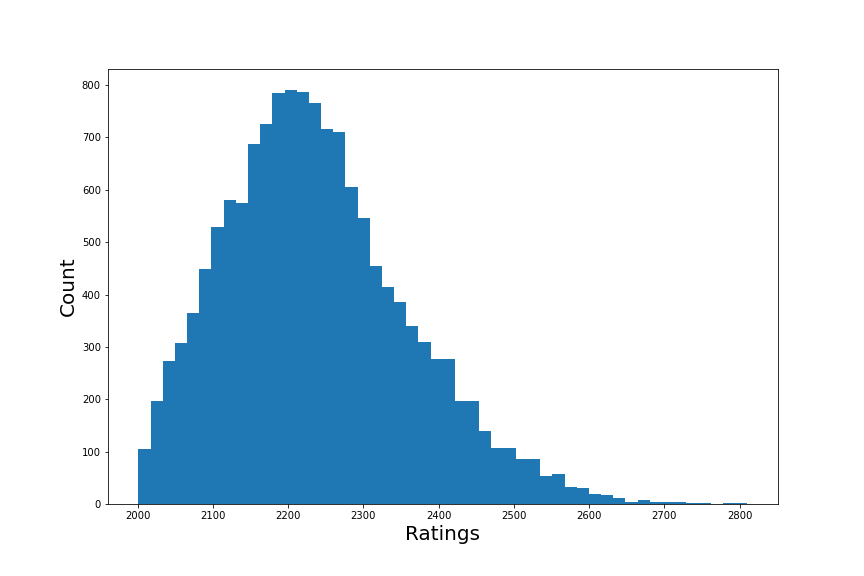
\includegraphics[width=\linewidth]{../figures/LiChessFigs/ratings_hist.png}
	
\end{figure}

[1] The ratings of the players in this pool ranges from 2000-2800, which is a very strong pool relative even to the population that plays chess.

\pagebreak

\begin{figure}[hbp]

	\centering 
	
	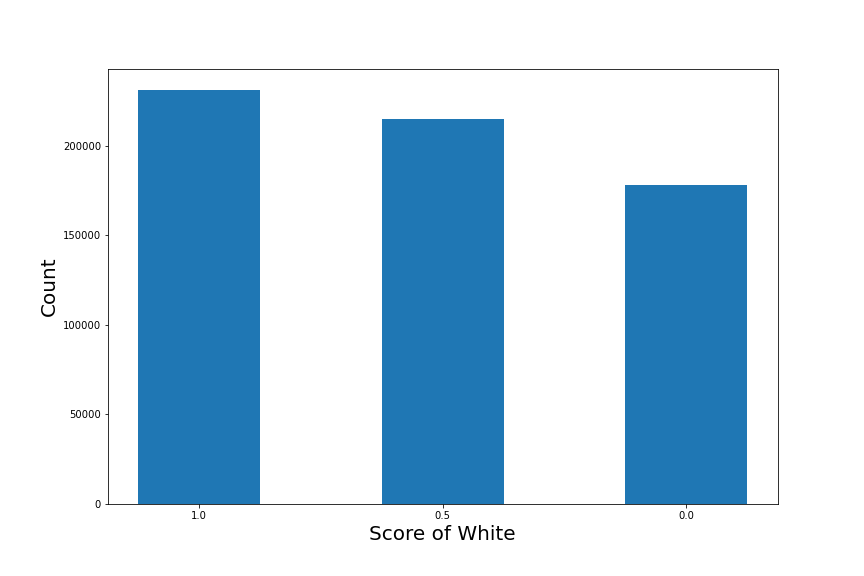
\includegraphics[width=\linewidth]{../figures/LiChessFigs/white_win.png}

\end{figure}

[2] In the first 96 months of the dataset, white wins a greater percentage of games than black.

\pagebreak

\begin{figure}[hbp]

	\centering
		
	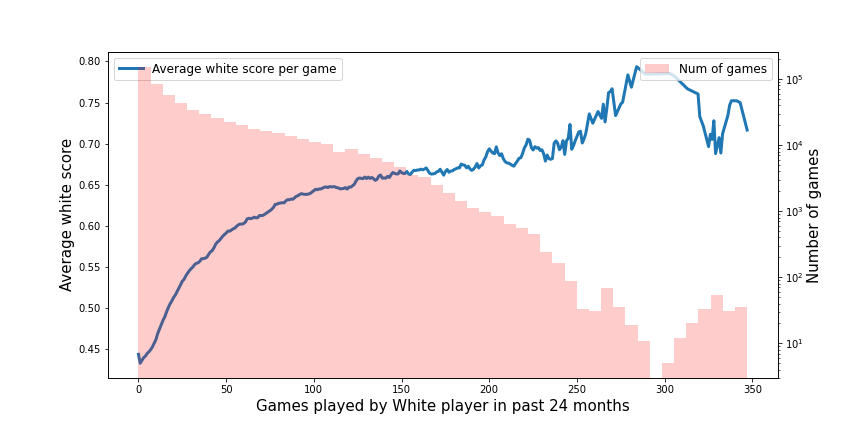
\includegraphics[width=\linewidth]{../figures/LiChessFigs/white_pre.png}
	
	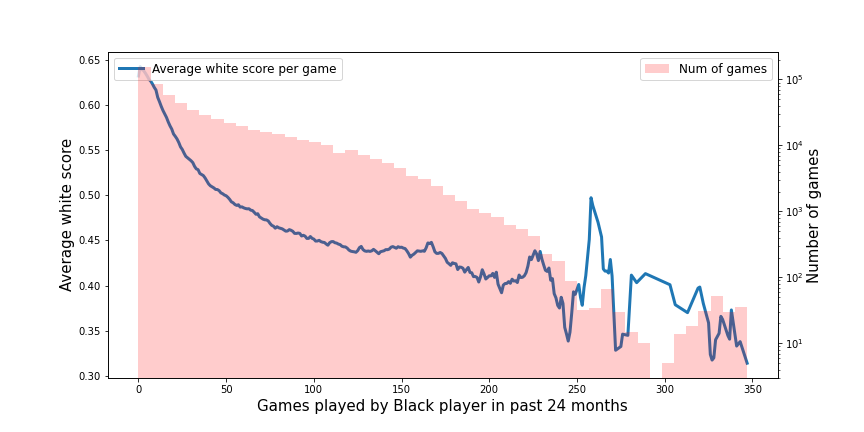
\includegraphics[width=\linewidth]{../figures/LiChessFigs/black_pre.png}
	
\end{figure}

[3] The average score the white player earns per game rises with the experience of the white player, and drops with the experience of the black player.

\end{document}